\section{Models}

\begin{frame}{Overview}
	\begin{itemize}
		\item Single-Encoder Approach
		\item Multi-Encoder Approach
		\begin{itemize}
			\item Integration Outside the Decoder
			\item Integration Inside the Decoder
			\begin{itemize}
				\item Sequential Attentions
				\item Parallel Attentions
			\end{itemize}
		\end{itemize}
	\end{itemize}
\end{frame}

\begin{frame}{Multi-Encoder - Integration Outside the Decoder}
	\begin{figure}
		\centering
		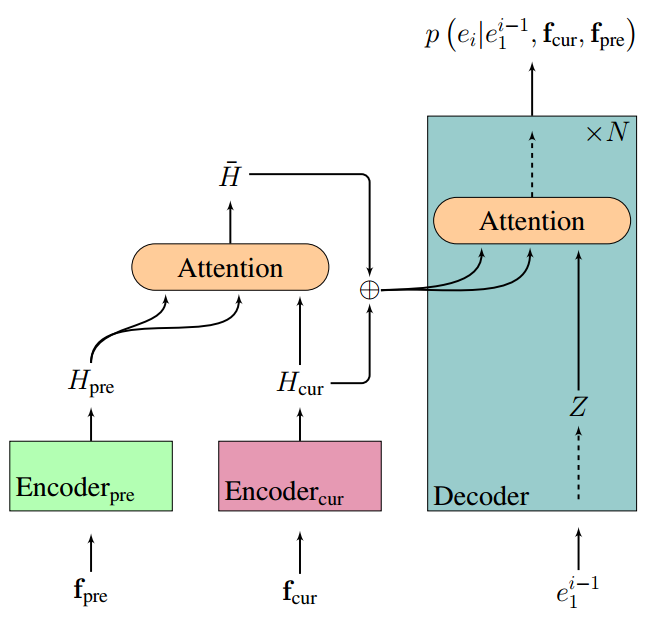
\includegraphics[width=0.53\linewidth]{Images/models_outide_decoder}
		\caption{}
		\label{fig:modelsoutidedecoder}
	\end{figure}
\end{frame}

\begin{frame}{Multi-Encoder - Integration Outside the Decoder}

\cite{maruf_document_2018} \textbf{Two-pass approach \textcolor{red}{(not training! to explain...)}. All context (source and target). Fr/De/Et$\to$En. Decoder without attention (integration in the RNN gates).} First pass for sentence representations (filling the memories), second pass for integrating current sentence representation with information stocked into memories (via coarse attention). \textcolor{red}{extention: attention to target memory!}
FORSE VA MESSO NELLA SEZIONE CACHES

\end{frame}


\begin{frame}{Multi-Encoder - Integration Outside the Decoder}
	\begin{itemize}
		\item encoders might encode multiple previous sentences. E.g. \cite{wang_exploiting_2017}.
		\item architectures might be RNNs (e.g. \cite{wang_exploiting_2017}) or Transformers (e.g. \cite{zhang_improving_2018})
		\item integration inside the decoder might happen with a different system than cross-attention. E.g. \cite{wang_exploiting_2017} propose to concatenate the context representation to the cell state of the decoder's RNN.
		\item source-side attention to context can be at both sentence and word level. E.g. \cite{maruf_selective_2019, miculicich_document-level_2018}.
		\item gating context is a way substitutes residual add.
		\item despite some have considered target-side context harmful because of the \textit{error propagation} problem \cite{zhang_improving_2018}, now...
		\item weight sharing is blabla \cite{voita_context-aware_2018}. Some use it. In general, it has been proven to be successful by a comparative study \cite{yamagishi_improving_2019}.
		\item two-step training what is. E.g. \cite{zhang_improving_2018, miculicich_document-level_2018}. Explain that DL training corpus is small! possible future direction...
	\end{itemize}
\end{frame}

\begin{frame}{Multi-Encoder - Integration Outside the Decoder}
	\begin{table}
		\begin{tabular}{ *{5}{c|} c }

			\thead{Reference}
			& \thead{Context}
					& \thead{Two-Pass\\ Approach}
						& \thead{Outside\\ Integr.}
							& \thead{Inside\\ Integr.}
								& \thead{Lang.\\ Pair}
									 \\
			\hline\hline
			\cite{wang_exploiting_2017}&s:-3 &&optional&optional&Zh$\to$En\\
			\hline
			\cite{voita_context-aware_2018}&s:-1&&yes&&En$\to$Ru\\
			\hline
			\cite{zhang_improving_2018}&s:-2&&yes&sequential&Zh$\to$En\\
			\hline
			\cite{miculicich_document-level_2018}&s:-3; t:-3&&yes&&Zh/Es$\to$En\\
			\hline
			\cite{maruf_selective_2019}&s:all; t:all&optional&yes&&En$\to$De\\
			\hline
			\cite{jean_does_2017}&s:-1&&&parallel&En$\to$De/Fr\\
			\hline
			\cite{bawden_evaluating_2018}&s:-1; t:-1&&&parallel&En$\to$Fr\\
			\hline
			\cite{fu_reference_2019}&s:all; t:-1&yes&&parallel&En/Zh$\to$De/En\\
			\hline
		\end{tabular}
	\end{table}
\end{frame}

\begin{frame}{Multi-Encoder - Integration Inside the Decoder}
	\begin{figure}
		\centering
		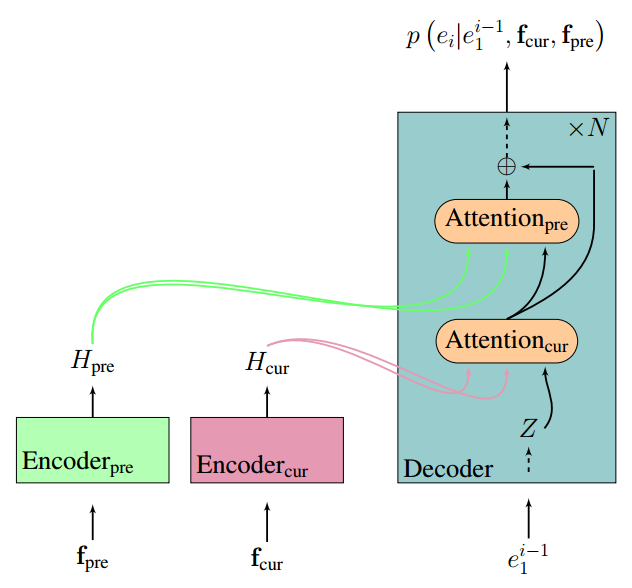
\includegraphics[width=0.5\textwidth]{Images/models_inside_decoder_sequential}%
		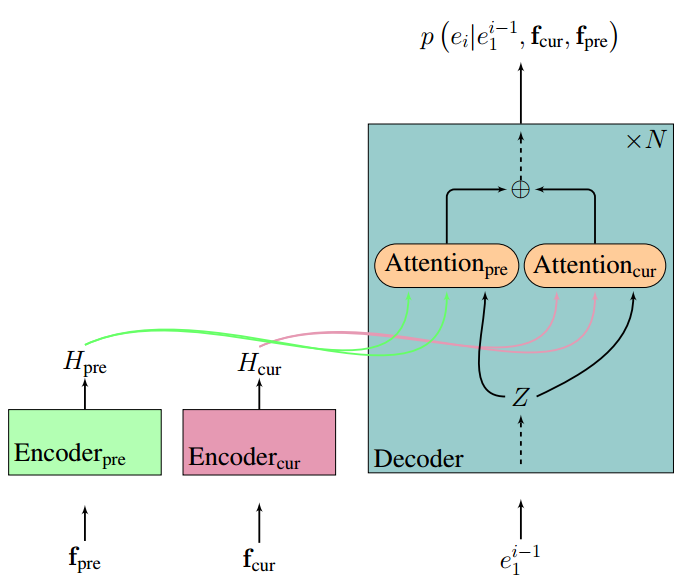
\includegraphics[width=0.5\textwidth]{Images/models_inside_decoder_parallel}
		\caption{}
		\label{fig:modelsinsidedecodersequential}
	\end{figure}
\end{frame}


%%%%%%%%%%%%%%%%%%%%%%%%%%%%%%%%%%%%%%%%%%%%%%%%%%%%%%%%%%%%%%%%%%%%%%%%%

\subsection{Remarks and conclusions}

\begin{frame}{Remarks and conclusions}
	\textbf{Possible Future Research Directions}
	\begin{itemize}
		\item build a large DL corpus for training systems;
	\end{itemize}
\end{frame}

%\begin{frame}{Regret}
%
%	\begin{columns}
%	\begin{column}{0.6\textwidth}
%	 \onslide<+->\begin{block}{Sub-linear Regret}
%	\begin{enumerate}
%			\item<+-|alert@+> for any linear function $f(T)$, for sufficiently large input $T$, $Regret(T)$ grows slower than $f(T)$.
%			\item<+-|alert@+> Alternatively, $\lim_{T\to\infty}Regret(T)/T=0$
%		\end{enumerate}
%	\end{block}
%	\end{column}
%
%	\begin{column}{0.4\textwidth}
%		\centering
%		\includegraphics<+->[width=1\textwidth]{Images/mabomber}
%	\end{column}
%	\end{columns}
%\end{frame}


%\begin{frame}{A useful formulation}
%
%	\begin{columns}
%	\begin{column}{0.4\textwidth}
%	  \begin{center}
%	     \includegraphics<+->[width=1\textwidth]{Images/mabomber}
%	  \end{center}
%%	    \quad Multi \hspace{0.80cm} Armed \hspace{0.70cm} Bandits
%	\end{column}
%
%	\begin{column}{0.6\textwidth}
%	\begin{block}{Multi Armed Bandits}
%	    \begin{itemize}
%	    \item<+-|alert@+> Simpler framework;
%	    \item<+-|alert@+> Share the exploration-exploitation tradeoff;
%	    \item<+-|alert@+> Ample literature available.
%	    \end{itemize}
%	 \end{block}
%	 
%	 \onslide<+->{	
%	\begin{block}{Regret}
%	 $Regret(T)=\mathcal{O}(\sqrt T)\to$ regret is \textbf{sub-linear}.
%	\end{block}
%	}
%	
%%	\onslide<+->{	
%%	\begin{block}{Desideratum}
%%	 \textbf{sub-linear} $Regret(T)\Leftrightarrow \lim_{T\to\infty}Regret(T)/T=0$
%%	 \\~\\
%%	 E.g. $Regret(T)=\mathcal{O}(\log T)$
%%	\end{block}
%%	}
%%	
%	\end{column}
%	\end{columns}
%\end{frame}


%	\onslide<2->{
%	\textbf{Rewards}: portfolio log-return with transaction costs
%		\begin{equation*}
%			R_{t+1} = \log \left\{ 1 + \sum^{I}_{i=0} \left[ 
%				\tikz[baseline]{
%		        	\node[anchor=base] (t1) {$a_t^i X_{t+1}^i$};
%		        } - 
%		        \tikz[baseline]{
%		        	\node[anchor=base] (t2) {$\delta_i \left| a_t^i - \widetilde{a}_t^i \right|$};
%		       	} -
%		       	\tikz[baseline]{
%		       		\node[anchor=base] (t3) {$\delta_s {(a_t^i)}^-$};
%		       	} \right] -
%		       	\tikz[baseline]{
%		       		\node[anchor=base] (t4) {$\delta_f \mathbf{1}_{{a}_t \neq \tilde{{a}}_{t-1}}$};
%		       	} \right\}	 	
%		 \end{equation*}
%	}
%	
%	\onslide<7->{
%	\textbf{Actions}: Portfolio weights
%		\begin{equation*}
%			\{a_t^i\}_{i=0}^I \;\;\; \text{s.t.}\;\;\; \sum^{I}_{i=0} a_t^i = 1 \;\;\;\;\; \forall t \in \{0, 1, 2, \ldots\}
%		\end{equation*}
%	}
%
%	\onslide<8->{
%	\textbf{States}: assets past returns and current allocation
%		\begin{equation*}
%			S_t = \{X, X_t, X_{t-1}, \ldots, X_{t-P}, \tilde{a}_t\}
%		\end{equation*}
%	}
%	
%	\onslide<3|handout:0>{
%		\begin{tikzpicture}[overlay]
%				\node[draw=SteelBlue, circle, line width=3pt, minimum size=2cm] at (t1) {};
%		\end{tikzpicture}
%	}
%	
%	\onslide<4|handout:0>{
%		\begin{tikzpicture}[overlay]
%				\node[draw=SteelBlue, circle, line width=3pt, minimum size=2cm] at (t2) {};
%		\end{tikzpicture}
%	}
%		
%	\onslide<5|handout:0>{
%		\begin{tikzpicture}[overlay]
%				\node[draw=SteelBlue, circle, line width=3pt, minimum size=2cm] at (t3) {};
%		\end{tikzpicture}
%	}
%			
%	\onslide<6|handout:0>{
%		\begin{tikzpicture}[overlay]
%				\node[draw=SteelBlue, circle, line width=3pt, minimum size=2cm] at (t4) (g) {};
%		\end{tikzpicture}
%	}
%\end{frame}
%
%\begin{frame}[c]{Synthetic Asset: Convergence}
%\begin{figure}[t!]
%	\centering
%	\includegraphics[height=5cm,width=0.8\textwidth]{Images/6_0_single_synthetic_neutral_convergence}
%\end{figure}
%\end{frame}
%
%
%\begin{frame}[c]{Synthetic Asset: Backtest Performance}
%\begin{figure}[t]
%	\centering
%	\includegraphics[height=6cm,width=0.8\textwidth]{Images/6_1_single_synthetic_neutral_performance}
%\end{figure}
%\end{frame}
%
%\begin{frame}[c]{Synthetic Asset: Impact of Transaction Costs}
%\begin{figure}[t!]
%	\centering
%	\includegraphics[height=3cm,width=0.8\textwidth]{Images/6_2_impact_transaction_costs}
%\end{figure}
%\begin{figure}[t!]
%	\centering
%	\includegraphics[height=3cm,width=0.8\textwidth]{Images/6_3_impact_short_selling_fees}
%\end{figure}
%\end{frame}
%
%\begin{frame}{Not So Fast}
%
%	\onslide<1->{
%	\begin{columns}
%	\begin{column}{0.6\textwidth}
%	   \begin{alertblock}{Insuccess on Historical Data}
%	   Successfully applying these RL algorithms to historical data is much more challenging
%	   \begin{enumerate}
%	   		\item Fail to converge
%	   		\item The strategies learned are not profitable
%	   \end{enumerate}
%	   \end{alertblock}
%	\end{column}
%	\begin{column}{0.4\textwidth}
%	    \begin{center}
%	     \includegraphics[width=1\textwidth]{Images/8_9_single_hist_neutral_performance}
%	     \end{center}
%	\end{column}
%	\end{columns}
%	}
%	
%	\onslide<2->{	
%	\begin{block}{Possible Explanations}
%		\begin{enumerate}
%			\item<2-> \textbf{Low signal-to-noise ratio}: extremely difficult to find tradable patterns in markets
%			\item<3-> \textbf{Quality of data}: unlikely to find patterns in daily prices of liquid stocks
%			\item<4-> \textbf{Weak features}: parametric policy must be powerful enough to capture the signal
%			\item<5-> \textbf{Non-stationarity of financial time-series}: a signal needs to be persistent
%		\end{enumerate}
%	\end{block}
%	}

